\documentclass{rapportENSIAS}

\usepackage{booktabs}
\usepackage{longtable}
\usepackage{array}
\usepackage{enumitem}
\usepackage{xcolor}
\usepackage{listings}
\usepackage{microtype}
\usepackage{csquotes}

\definecolor{codebg}{rgb}{0.96,0.96,0.96}
\definecolor{janusblue}{RGB}{30,79,125}
\lstset{
  basicstyle=\ttfamily\small,
  backgroundcolor=\color{codebg},
  frame=single,
  breaklines=true,
  columns=fullflexible,
  showstringspaces=false
}
\hypersetup{
  colorlinks=true,
  linkcolor=janusblue,
  citecolor=janusblue,
  urlcolor=janusblue,
  pdftitle={JANUS: AI-Assisted Honey Documents for Deception and Attacker Interaction Detection}
}
\graphicspath{{figures/}{figures/evidence/}}

\newcommand{\plannedfigure}[3]{
  \begin{figure}[H]
    \centering
    \IfFileExists{#1}{
      \includegraphics[width=0.94\linewidth]{#1}
    }{
      \fbox{\parbox[c][5.0cm][c]{0.88\linewidth}{\centering
        Figure to be exported from Mermaid source:\\[0.4em]
        \texttt{#1}}}
    }
    \caption{#2}
    \label{#3}
  \end{figure}
}

\title{JANUS Final Year Project Report}

\begin{document}

\titre{JANUS: AI-Assisted Honey Documents for Deception and Attacker Interaction Detection}
\sujet{Final Year Project}
\UE{Cybersecurity, Cloud and Mobile Computing}
\enseignant{[Supervisor name]}
\eleves{[Student name(s)]}
\jury{[Jury members]}
\annee{2025-2026}

\fairemarges
\fairepagedegarde

\pagenumbering{roman}

\chapter*{Acknowledgements}
\addcontentsline{toc}{chapter}{Acknowledgements}
This section will be completed by the student. It should thank the project
supervisor, the jury, the ENSIAS teaching staff, and the people who directly
supported the work, without using generic or invented names.

\chapter*{Abstract}
\addcontentsline{toc}{chapter}{Abstract}
JANUS is a defensive cyber-deception prototype that generates realistic
honey documents with artificial intelligence, deploys them in a monitored
directory, and correlates local endpoint evidence with remote Canarytokens
signals. The project addresses a practical limitation of static honey files:
their content rapidly becomes repetitive, while a single remote callback does
not explain what happened on the monitored host. JANUS therefore combines a
controlled generation pipeline, artifact safety gates, Windows System Access
Control List auditing, Wazuh rules and collection, official Canarytokens, an
SQLite evidence registry, and a Streamlit dashboard. The implemented formats
include DOCX, XLSX, CSV, JSON, YAML, ENV, and ZIP. Tests performed on Windows
show that a file read can be traced to Security event 4663 and a dedicated
Wazuh rule while preserving the original evidence. Office and AWS tokens add a
remote signal when their format-specific activation condition is met. The
prototype deliberately avoids claims that cannot be supported: an Internet
callback normally exposes an egress IP rather than a device identity, a MAC
address is unavailable across routed networks, and one read event alone does
not prove a remote download. The result is a reproducible academic MVP that
demonstrates defense-in-depth for honey documents and documents its operational
and forensic limits.

\vspace{0.5em}
\noindent\textbf{Keywords:} cyber deception, honey document, honeytoken,
Wazuh, Canarytokens, Windows auditing, generative AI, digital evidence.

\chapter*{List of Abbreviations}
\addcontentsline{toc}{chapter}{List of Abbreviations}
\begin{longtable}{>{\bfseries}p{0.18\linewidth}p{0.72\linewidth}}
API & Application Programming Interface \\
AWS & Amazon Web Services \\
FIM & File Integrity Monitoring \\
HIDS & Host-based Intrusion Detection System \\
LLM & Large Language Model \\
MVP & Minimum Viable Product \\
OOXML & Office Open XML \\
SACL & System Access Control List \\
SIEM & Security Information and Event Management \\
SOC & Security Operations Center \\
TTP & Tactic, Technique, and Procedure \\
TTL & Time To Live \\
\end{longtable}

\clearpage
\tabledematieres
\listoffigures
\clearpage
\listoftables
\clearpage

\pagenumbering{arabic}
\chapter*{General Introduction}
\addcontentsline{toc}{chapter}{General Introduction}
Organizations protect sensitive documents with access controls, endpoint
monitoring, and data-loss prevention. These mechanisms remain necessary, but
they mostly react to access involving known assets. A well-placed decoy creates
a different signal: because the file has no legitimate operational purpose,
an interaction with it has a high investigative value. The challenge is not
only to create an attractive filename. A useful honey document must remain
credible, must not leak real secrets, must be deployable at scale, and must
produce evidence that an analyst can interpret without overclaiming.

JANUS explores this problem through two complementary observation layers. The
first is local: Windows auditing and Wazuh record the account, process, object
path, access mask, and event time on a monitored endpoint. The second is
remote: a Canarytoken can notify the defender when Office loads external
content or when decoy cloud credentials are presented to the AWS API. An
AI-assisted generation stage provides varied business content, while safety
checks and format-specific assemblers keep the artifacts controlled.

This report presents the problem, related technologies, requirements,
architecture, implementation, validation, and limitations of the resulting
prototype. Particular attention is given to evidence quality: direct
observations are separated from inferences, and unavailable attacker
attributes are never fabricated.

\chapter{Project Context and Problem Definition}

\section{Introduction}

Cybersecurity monitoring usually concentrates on production resources: user
accounts, servers, business applications, and sensitive data. This produces a
large volume of legitimate activity that analysts must distinguish from
malicious behavior. Cyber deception changes this asymmetry by introducing
resources that have no normal business use. When such a resource is accessed,
the event deserves immediate investigation. NIST includes deception and
honeytokens among the techniques that can support cyber-resilient systems
\cite{nist800160v2}.

JANUS focuses on a specific deception resource: the honey document. Examples
include a financial workbook, an internal procedure, a technical configuration,
or decoy cloud credentials. The file must be sufficiently plausible to attract
an intruder, while remaining harmless and distinguishable from real data by the
defender.

\section{Problem statement}

A static decoy file is easy to deploy, but it presents four practical
limitations.

\begin{enumerate}[label=\arabic*.]
  \item \textbf{Limited realism and diversity.} Reusing the same names and
  content makes a deception environment easier to fingerprint.
  \item \textbf{Incomplete observation.} A remote callback can show that a
  token endpoint was contacted, but it does not by itself explain which local
  account and process touched the file.
  \item \textbf{Format-dependent activation.} A Word beacon, an Excel token,
  a web breadcrumb, and AWS decoy credentials do not activate in the same way.
  \item \textbf{Risk of unsupported conclusions.} An event may identify a
  process or an egress IP without proving a person's identity, a device MAC
  address, or a complete attack path.
\end{enumerate}

The central question is therefore:

\begin{quote}
How can a defensive platform generate credible and controlled honey documents,
deploy them safely, and combine local and remote evidence to detect attacker
interaction without fabricating unavailable attributes?
\end{quote}

\section{Research questions}

The project is structured around the following questions:

\begin{itemize}
  \item How can an LLM vary business content without receiving local paths,
  secrets, or live token material?
  \item Which Canarytoken type is appropriate for each generated file format?
  \item Which Windows and Wazuh fields are direct evidence of file access?
  \item How can raw Wazuh evidence, normalized events, and verdicts remain
  traceable to one HoneyDoc instance?
  \item Which claims about the attacker are reliable, inferred, or impossible?
\end{itemize}

\section{Objectives}

\subsection{Primary objective}

The primary objective is to implement a reproducible MVP that joins four
capabilities: AI-assisted content generation, format-specific tokenization,
controlled deployment, and evidence correlation.

\subsection{Functional objectives}

\begin{itemize}
  \item Generate financial, human-resources, technical, and cloud-credential
  decoys in DOCX, XLSX, CSV, JSON, YAML, ENV, and ZIP formats.
  \item Create official Canarytokens only after the content passes safety and
  coherence checks.
  \item Deploy files atomically under a single authorized root and record their
  SHA-256 hashes in SQLite.
  \item Detect local read, modification, and deletion events using Windows
  auditing and Wazuh rules.
  \item Preserve raw Wazuh alerts and expose normalized fields through an
  authenticated API and dashboard.
  \item State token activation conditions and sensor limitations in the user
  interface.
\end{itemize}

\subsection{Security and quality objectives}

The system must avoid macros by default, prevent path traversal, keep
administrative routes behind an API key, avoid printing secret token material,
and fail closed when the configured Canarytokens provider is unavailable.
Tests must cover artifact structure, database migration, API security,
deployment policy, token-provider behavior, Wazuh parsing, verdict generation,
and dashboard navigation.

\section{Scope and non-goals}

The supported core contains the HoneyDoc pipeline, Wazuh, Canarytokens, SQLite,
FastAPI, and Streamlit. Experimental fake SSH and HTTP services are excluded
from the validated architecture because they depend on a later attacker choice
to reuse exposed credentials; they do not improve the initial observation of a
document interaction. Prompt-injection and credential-trap layers also remain
disabled by default.

The project is not a production SOC platform. It does not provide high
availability, immutable storage, global endpoint coverage, attribution of a
human identity, or retrieval of a remote MAC address. Wazuh observes only hosts
on which an agent and the required audit policy are active. A Canarytokens hit
can continue to work after a file leaves the monitored host, but its source IP
may be a proxy, VPN, NAT gateway, or security service.

\section{Methodology}

The implementation followed an incremental engineering process:

\begin{enumerate}[label=\arabic*.]
  \item establish a minimal DOCX generation and callback flow;
  \item configure a project-local monitored directory and inherited SACL;
  \item validate Windows event 4663 and dedicated Wazuh rules;
  \item generalize registration and correlation to every active HoneyDoc;
  \item add XLSX and structured formats with explicit token policies;
  \item integrate the official Canarytokens provider;
  \item preserve raw and normalized evidence in SQLite;
  \item add a unified dashboard and automated regression tests;
  \item perform manual Office, Canary email, and end-to-end Wazuh tests.
\end{enumerate}

\section{Contributions}

The main contributions of JANUS are:

\begin{itemize}
  \item a multi-format generation pipeline that separates narrative generation
  from artifact assembly;
  \item a token policy that reflects real activation semantics instead of
  promising an automatic callback for every file;
  \item an Office beacon implementation compatible with an external OOXML image
  relationship and requiring no macro;
  \item a local detection path from SACL and event 4663 to Wazuh and a JANUS
  verdict;
  \item a chain of evidence linking raw alert hashes, normalized signals, and
  HoneyDoc registry entries;
  \item a dashboard that visibly separates Wazuh observations from remote
  Canarytokens callbacks.
\end{itemize}

\section{Report organization}

Chapter 2 reviews the relevant deception, auditing, Wazuh, Canarytokens, and AI
concepts. Chapter 3 defines requirements and presents the architecture. Chapter
4 details the implementation and validation. Chapter 5 analyzes evidence
quality, limitations, security hardening, and future work.

\section{Conclusion}

The project is motivated by a simple principle: a decoy is useful only when its
interaction is observable and its evidence is interpreted honestly. The next
chapter positions JANUS among the technologies that implement this principle.


\chapter{State of the Art and Technical Foundations}

\section{Introduction}

JANUS combines technologies that are often deployed independently. Honeytokens
provide low-noise tripwires, host auditing records local activity, a SIEM/HIDS
normalizes evidence, and generative AI varies the decoy content. This chapter
explains the role and limits of each component.

\section{Cyber deception and honey documents}

Cyber deception deliberately exposes false information or services in order to
influence an adversary and improve defender observation. In contrast with a
production resource, a properly isolated decoy should have no routine use. This
raises the investigative value of an interaction, but it does not automatically
make every event malicious: antivirus, indexing software, backup agents, and
authorized tests can also touch a file. A mature design therefore records
context and supports suppression rather than assuming intent from one event.

A honey document is a decoy file with a plausible business purpose and one or
more observation mechanisms. Its realism depends on its filename, internal
structure, metadata, placement, and consistency with neighboring files. Its
safety depends on the absence of real secrets and dangerous active content.

\section{Honeytokens and remote callbacks}

Canarytokens implement lightweight tripwires that notify a defender when a
unique token is used. The official getting-started guide describes the basic
model as create, place, and wait for an alert \cite{canaryGettingStarted}.
Activation is token-specific.

\subsection{Office tokens}

Microsoft Word and Excel tokens can alert when opened in their native
applications \cite{canaryOffice}. Non-macro variants rely on a network lookup
for embedded external content. This is preferable for JANUS because it avoids
asking users to enable macros. It is nevertheless conditional: protected view,
external-content policy, offline operation, or network filtering can prevent
the request.

\subsection{Web breadcrumbs}

A URL embedded in CSV, JSON, YAML, ENV, or ZIP content is passive. Opening the
file in a text editor does not execute a network request. The alert occurs only
if a person or tool uses the URL. JANUS therefore labels this mode as
user-action-required instead of automatic.

\subsection{AWS key tokens}

An AWS API Keys Canarytoken is a decoy access-key pair. Thinkst documents that
an alert is generated when the keys are used through the AWS API and notes a
possible delay of 2 to 30 minutes through AWS logging infrastructure
\cite{canaryAws}. Merely displaying an ENV file must not be reported as a
remote token activation.

\section{Windows SACL and event 4663}

A System Access Control List specifies which access attempts on a securable
object must be audited. It is distinct from a discretionary ACL: the SACL does
not grant access; it requests audit records when selected rights are exercised.

Windows Security event 4663 states that an operation was performed on an
object. Microsoft explains that it is generated only when the object's SACL
contains the required audit entry and that, unlike event 4656, it represents a
right that was used rather than merely requested \cite{microsoft4663}. Useful
fields include:

\begin{itemize}
  \item \texttt{ObjectName}: the accessed file or directory;
  \item \texttt{ProcessName} and \texttt{ProcessId}: the local process;
  \item \texttt{SubjectUserName}, domain, SID, and logon ID: the security
  context;
  \item \texttt{AccessMask} and \texttt{AccessList}: the exercised rights;
  \item timestamp, computer name, and event record identifier.
\end{itemize}

Event 4663 is strong evidence that a right was exercised on the monitored host,
but it is not a semantic record of user intention. A read can result from Word,
PowerShell, an antivirus engine, an indexer, or a copy utility. A remote
download requires corroborating SMB, authentication, process, or network
events.

\section{Wazuh file and event monitoring}

Wazuh provides agent-based collection, rules, indexing, and visualization.
Its File Integrity Monitoring module tracks file creation, modification, and
deletion by comparing checksums and attributes \cite{wazuhFim}. In who-data
mode on Windows, Wazuh uses the Microsoft audit subsystem and can configure the
required audit policy and SACL \cite{wazuhWhodata}. JANUS additionally consumes
the Security event channel and applies dedicated rules to audited access under
the project deployment root.

For Linux, the kernel audit system can monitor read, write, execute, and
attribute access using keyed audit rules; Wazuh provides a documented path for
collecting and visualizing these events \cite{wazuhAuditd}. JANUS includes an
adapter for Linux audit signals, but the validated demonstration environment is
Windows.

\section{Generative AI for deception content}

An LLM can produce varied business narratives and reduce the repetitive nature
of static templates. It should not directly control deployment, token creation,
or filesystem paths. JANUS therefore uses the model for constrained text only.
Deterministic code selects the format, creates the token, assembles the file,
validates its structure, chooses the destination, and records evidence. A local
fallback keeps the project testable when a remote model is not configured.

The main risks are leakage of secrets in prompts, uncontrolled model output,
hallucinated operational claims, prompt injection embedded in source material,
and non-reproducible content. The implementation addresses these risks through
prompt minimization, a controlled corpus, coherence checks, forbidden-pattern
scanning, and post-generation artifact validation.

\section{Comparative analysis}

\begin{table}[H]
\centering
\caption{Comparison of observation mechanisms used by JANUS}
\label{tab:mechanism-comparison}
\small
\begin{tabular}{p{0.19\linewidth}p{0.24\linewidth}p{0.24\linewidth}p{0.24\linewidth}}
\toprule
Mechanism & Direct evidence & Main value & Main limitation \\
\midrule
Windows 4663 & Account, process, object, access right, time & Local interaction context & Only on an audited host; read semantics are limited \\
Wazuh & Normalized alert, rule, agent, indexed evidence & Collection and correlation & Depends on agent, rules, and indexer availability \\
Office token & Remote HTTP/DNS activation and request metadata & Detection after the file leaves the host & Can be blocked by Office or network policy \\
AWS keys token & Use of a decoy key against AWS APIs & High-value credential-use signal & Opening the file does not activate it; alert may be delayed \\
Web breadcrumb & Request to a unique URL & Simple cross-platform tripwire & Requires a deliberate click or tool action \\
\bottomrule
\end{tabular}
\end{table}

\section{Positioning of JANUS}

JANUS is not a replacement for Wazuh or Canarytokens. Its contribution is the
orchestration layer between them: it generates and registers each decoy,
selects the appropriate token, controls deployment, correlates endpoint events
with the active registry, and explains sensor limits in one interface. The
design is intentionally low interaction and defensive.

\section{Conclusion}

No single sensor provides every desired attacker attribute. The architecture
must combine endpoint evidence and remote tripwires while preserving the
different confidence levels of each source. Chapter 3 turns these principles
into system requirements and components.


\chapter{Requirements, Design, and Architecture}

\section{Introduction}

This chapter translates the evidence and safety principles into an architecture
that can be implemented and tested. The design separates preparation of the
decoy from observation of an interaction, and it isolates format-dependent
behavior behind explicit policies.

\section{Actors and use cases}

Three actors interact with the core system:

\begin{itemize}
  \item the \textbf{defender/operator}, who configures JANUS, generates decoys,
  and investigates signals;
  \item the \textbf{local or remote actor}, who discovers, opens, modifies,
  moves, deletes, or uses a decoy;
  \item external \textbf{sensor services}, namely Wazuh and Canarytokens, which
  produce complementary evidence.
\end{itemize}

\plannedfigure{figures/system-context.png}
{JANUS system context and external actors}{fig:system-context}

\section{Functional requirements}

\begin{table}[H]
\centering
\caption{Main functional requirements}
\label{tab:functional-requirements}
\small
\begin{tabular}{p{0.12\linewidth}p{0.79\linewidth}}
\toprule
ID & Requirement \\
\midrule
FR-01 & Generate a HoneyDoc for an authorized business type and output format. \\
FR-02 & Select a compatible official token type and document its activation condition. \\
FR-03 & Reject unsafe, incoherent, or unsupported content before token creation and deployment. \\
FR-04 & Restrict deployment to the configured project-local root. \\
FR-05 & Register the artifact, token metadata, hash, TTL, and deployment path in SQLite. \\
FR-06 & Collect Wazuh alerts, correlate them with active HoneyDocs, and normalize the action. \\
FR-07 & Preserve raw evidence and a deterministic SHA-256 evidence hash. \\
FR-08 & Display local Wazuh signals and remote Canarytokens callbacks separately. \\
FR-09 & Support controlled token retirement and HoneyDoc rotation. \\
\bottomrule
\end{tabular}
\end{table}

\section{Non-functional requirements}

\begin{itemize}
  \item \textbf{Safety:} generated artifacts contain no real secret and no
  macro; paths remain within the deployment root.
  \item \textbf{Traceability:} every signal can be linked to a HoneyDoc and to
  immutable raw evidence.
  \item \textbf{Honesty:} fields distinguish direct observation, inference,
  confidence, and unavailable data.
  \item \textbf{Security:} administrative API routes require an API key;
  secrets are excluded from Git and routine logs.
  \item \textbf{Reproducibility:} a local content fallback and automated tests
  keep the project runnable without a remote LLM.
  \item \textbf{Maintainability:} generators, token policy, deployment,
  collection, correlation, and presentation remain separate modules.
\end{itemize}

\section{Global architecture}

The system is divided into five logical planes:

\begin{enumerate}[label=\arabic*.]
  \item \textbf{Control plane:} FastAPI endpoints, authentication, configuration,
  and the Streamlit operator interface.
  \item \textbf{Generation plane:} corpus-based prompt construction, LLM or
  fallback content, coherence checks, token policy, and artifact assemblers.
  \item \textbf{Deployment plane:} authorized-path resolution, atomic writes,
  hashing, TTL, and the SQLite registry.
  \item \textbf{Observation plane:} Windows SACL/event 4663, Wazuh rules and
  Indexer, remote Canarytokens, and optional Linux audit telemetry.
  \item \textbf{Evidence plane:} raw alerts, normalized events, verdicts,
  timelines, and dashboard views.
\end{enumerate}

\plannedfigure{figures/detection-architecture.png}
{End-to-end JANUS generation and detection architecture}
{fig:detection-architecture}

\section{Generation pipeline}

The API receives a document type, format, scenario, target subdirectory, and
TTL. The deployment target is resolved before prompt construction so an
untrusted path cannot escape the allowed root. The LLM receives only business
context. Content is checked before a remote token is allocated. A deterministic
assembler then creates the requested file and a final gate inspects its
structure before deployment.

\plannedfigure{figures/generation-pipeline.png}
{Controlled HoneyDoc generation pipeline}{fig:generation-pipeline}

\subsection{Supported format policy}

\begin{table}[H]
\centering
\caption{Document types, formats, and remote activation}
\label{tab:format-policy}
\small
\begin{tabular}{p{0.22\linewidth}p{0.25\linewidth}p{0.20\linewidth}p{0.24\linewidth}}
\toprule
Document type & Formats & Token & Remote trigger \\
\midrule
Financial report & DOCX, XLSX, CSV, JSON & Word, Excel, or web & Office external content or breadcrumb use \\
HR document & DOCX, CSV, JSON & Word or web & Office external content or breadcrumb use \\
Technical configuration & DOCX, ENV, YAML, JSON, ZIP & Word or web & Office external content or breadcrumb use \\
Cloud credentials & ENV, YAML, JSON, ZIP & AWS keys & Decoy key used with AWS API \\
\bottomrule
\end{tabular}
\end{table}

\section{Local detection design}

The monitored directory is \texttt{data/shared}. A SACL entry inherited by
children requests successful audit events for read, create/write, append, and
delete rights. The Wazuh agent collects the Windows Security channel and the
manager applies rules scoped to this path.

\begin{table}[H]
\centering
\caption{JANUS Wazuh rule taxonomy}
\label{tab:wazuh-rules}
\small
\begin{tabular}{p{0.15\linewidth}p{0.28\linewidth}p{0.48\linewidth}}
\toprule
Rule & Normalized meaning & Interpretation \\
\midrule
100100 & Generic audited access & A 4663 event targets the monitored decoy root. \\
100101 & Read/open candidate & ReadData or equivalent was exercised. \\
100102 & Modification & WriteData or AppendData was exercised. \\
100103 & Deletion & Delete rights were exercised. \\
100104 & Office/PDF open candidate & A relevant application accessed the decoy. \\
100110 & Windows logon context & Candidate session context for correlation. \\
100111 & SMB access context & Candidate remote file-share context. \\
100112 & Process context & Relevant Windows process execution. \\
100130 & Linux command context & auditd/execve command signal. \\
\bottomrule
\end{tabular}
\end{table}

\section{Interaction sequence}

The sequence begins when an actor touches an active decoy. Windows emits the
audit event, the agent forwards it, Wazuh classifies it, and the JANUS collector
stores both raw and normalized evidence. Independently, a supported remote
token may activate. These paths can have different delays and are not forced
into one synthetic event.

\plannedfigure{figures/interaction-sequence.png}
{Sequence of a HoneyDoc interaction and evidence collection}
{fig:interaction-sequence}

\section{Registry and evidence model}

SQLite stores four related concepts:

\begin{itemize}
  \item a \textbf{HoneyDoc} instance with filename, path, type, format, hash,
  creation time, TTL, and active state;
  \item a \textbf{token} with provider, type, activation mode, callback metadata,
  and lifecycle state;
  \item a \textbf{Wazuh detection} with the Wazuh document/event identifiers,
  rule identifier, normalized action, process, user, and verdict;
  \item \textbf{raw evidence and security signals} linked by a canonical
  SHA-256 hash and correlation keys.
\end{itemize}

\plannedfigure{figures/evidence-data-model.png}
{Simplified registry and evidence data model}{fig:evidence-data-model}

\section{Trust boundaries and safeguards}

The principal trust boundaries are the LLM API, public Canarytokens service,
Wazuh Indexer, monitored filesystem, and administrative API. The LLM never
receives token secrets or the deployment path. The public token service receives
only the information required to create a token. Indexer credentials and the
JANUS API key remain in \texttt{.env}. Administrative responses avoid exposing
auth tokens and cloud secret material. The public webhook remains disabled
until a real HTTPS endpoint can authenticate and receive it.

\section{Conclusion}

The architecture treats generation, deployment, and observation as separate
security domains connected by explicit data contracts. Chapter 4 describes the
implementation and shows that these contracts hold in automated and live tests.


\chapter{Implementation and Validation}

\section{Introduction}

JANUS is implemented in Python and PowerShell around an existing Wazuh
single-node laboratory. FastAPI exposes the control surface, Streamlit provides
the dashboard, SQLite stores the registry and evidence, and Docker runs the
Wazuh manager, Indexer, and dashboard. The current validated host is Windows.

\section{Project structure}

\begin{lstlisting}[caption={Simplified JANUS source tree},label={lst:tree}]
HoneyDocJANUS/
|-- main.py
|-- src/
|   |-- alerting/        # FastAPI server and Streamlit dashboard
|   |-- core/            # configuration, database, evidence, safety
|   |-- janus/           # DOCX and multi-format generators
|   |-- janus_v2/        # registry, Wazuh, telemetry, verdicts
|   |-- lifecycle/       # atomic deployment and TTL rotation
|   `-- tactical/        # prompt, LLM, coherence and scoring
|-- scripts/             # setup, Wazuh rules, tests, start/stop
|-- corpus/              # controlled financial, HR and technical context
|-- data/shared/         # monitored deployment root (ignored by Git)
|-- docs/
`-- tests/
\end{lstlisting}

\section{Core implementation}

\subsection{Startup and configuration}

\texttt{main.py} initializes directories and the database, starts the FastAPI
application, and conditionally starts the rotation manager and experimental
components. Fake SSH/HTTP services and experimental prompt/credential layers
remain disabled. On application startup, the Wazuh detection collector and the
forensic collector are created only when their configuration is complete.

Configuration is loaded from \texttt{.env}; the real file is ignored by Git.
The API key protects administrative routes. Validation functions reject invalid
intervals, missing provider configuration in fail-closed mode, and unsafe path
settings.

\subsection{AI content and safety gate}

The tactical layer builds a business prompt from a controlled corpus. If a
remote LLM key is configured, the model returns a narrative; otherwise a local
fallback keeps the pipeline operational. The output passes a coherence check
and forbidden-pattern scan. Token allocation happens only after this gate,
which avoids wasting tokens or persisting external identifiers for rejected
content.

\subsection{DOCX assembly}

The DOCX generator writes visible business content and inserts a non-macro
Office beacon in the document footer. The OOXML contains one
\texttt{INCLUDEPICTURE} field and one external image relationship whose target
is the Word token URL. The final inspector opens the DOCX as a ZIP package and
requires exactly one matching field and relationship, no VBA parts, and no
visible JANUS fingerprint.

\subsection{XLSX and structured formats}

The accounting workbook generator creates balanced journal, income statement,
balance-sheet, and budget data. The workbook uses supported table/filter
structures and an external token reference that opens without Excel repair.
CSV, JSON, YAML, ENV, and ZIP generators create format-valid content and embed
only the token material allowed by policy. For cloud credentials, the provider's
exact decoy key pair is used; fallback fake fields are not invented.

\subsection{Deployment and registry}

The path policy resolves a requested target and rejects traversal outside
\texttt{JANUS\_DEPLOY\_ROOT}. The injector writes the artifact atomically,
computes SHA-256, and persists the document and token transaction. Generated
files, the database, logs, backups, and \texttt{.env} are excluded from Git.

\section{Wazuh and evidence processing}

PowerShell setup scripts configure the Windows audit subcategories, inherited
SACL, Wazuh manager rules, and Indexer collector settings. The collector queries
the configured rule set, handles overlap and search-after cursors, normalizes
4663 access masks into read/modify/delete, matches paths against active decoys,
and applies a deployment-grace suppression policy.

Every accepted alert is stored with Wazuh identifiers, the normalized action,
process, user, agent, verdict, raw JSON, and a canonical raw-evidence SHA-256.
The Wazuh rule identifier is also normalized into a top-level field so the
dashboard can display rules such as 100101 directly.

\section{Dashboard}

The Alert page intentionally presents two independent sections: local Wazuh
detections and Canarytokens callbacks received by JANUS. In the public
email-only configuration, the interface explains that provider emails are not
copied into the local callback table. A non-blocking Streamlit fragment refreshes
the alert view every five seconds without interfering with navigation.

The HoneyDocs page displays safe metadata only. The Generate page keeps the
dependent type and format selectors outside the submission form, preventing a
stale DOCX value after choosing JSON. It also explains the activation condition
before and after generation.

\section{Automated validation}

The final suite contains 98 tests and 7 subtests. It covers:

\begin{itemize}
  \item API authentication and callback rejection;
  \item path traversal and deployment-root enforcement;
  \item DOCX/XLSX beacon structure and absence of macros;
  \item structured format validity and ZIP path safety;
  \item Canarytokens provider selection and secret handling;
  \item SQLite migrations, registry, raw-evidence hashes, and cursor behavior;
  \item Wazuh parsing, collection, suppression, verdicts, and timelines;
  \item dashboard navigation and non-blocking refresh;
  \item local LLM fallback and coherence behavior.
\end{itemize}

The validated output is:

\begin{lstlisting}[caption={Automated acceptance result},label={lst:pytest}]
98 passed, 1 warning, 7 subtests passed
\end{lstlisting}

The remaining warning concerns a Starlette/httpx test-client deprecation and
does not represent a functional failure.

A final endurance check exposed contention between the Wazuh collector and the
forensic-retention transaction in the shared SQLite database. The collector
stores now use a common re-entrant writer lock, a 60-second busy timeout, and an
immediate retention transaction. A concurrent-writer regression test was added.
After an offline backup, bounded pruning, and vacuum, the database passed
\texttt{quick\_check}, retained all 130 Wazuh detections, and both collectors
completed successive polls with zero errors.

\section{Live Windows and Wazuh validation}

On 10 August 2026, the stack was restarted after a host reboot. Docker reported
the Wazuh manager, Indexer, and dashboard as running. The JANUS API, dashboard,
Wazuh collector, forensic collector, and Canarytokens provider all reported a
healthy state.

A controlled binary read of HoneyDoc 26 generated Windows Security event 4663.
Wazuh applied rule 100101, described as a JANUS read/open candidate. The JANUS
collector correlated the event with the active document and stored:

\begin{itemize}
  \item the audited object path and HoneyDoc identifier;
  \item action \texttt{read} and access mask \texttt{0x1};
  \item the PowerShell process and local test account;
  \item Wazuh rule identifier 100101;
  \item raw evidence and its SHA-256 hash;
  \item a low verdict because no expected host or expected user was configured.
\end{itemize}

\begin{figure}[H]
\centering
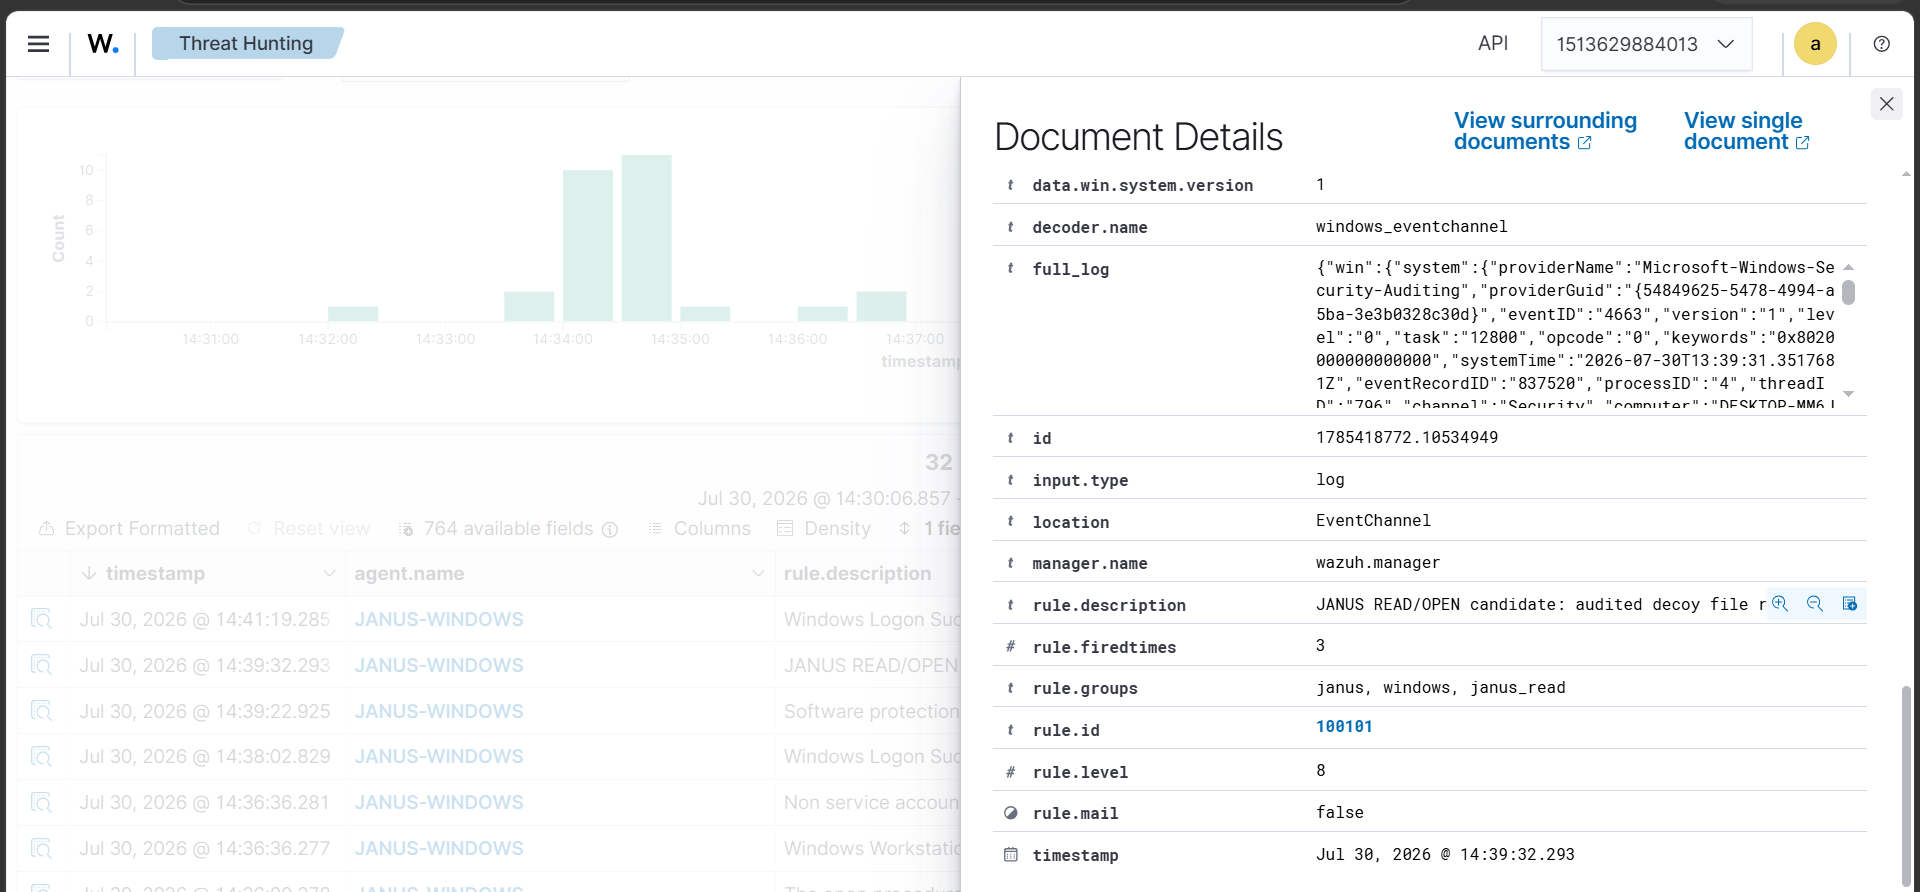
\includegraphics[width=0.95\linewidth]{wazuh-rule-100101.png}
\caption{Wazuh document details showing JANUS rule 100101}
\label{fig:wazuh-rule}
\end{figure}

\begin{figure}[H]
\centering
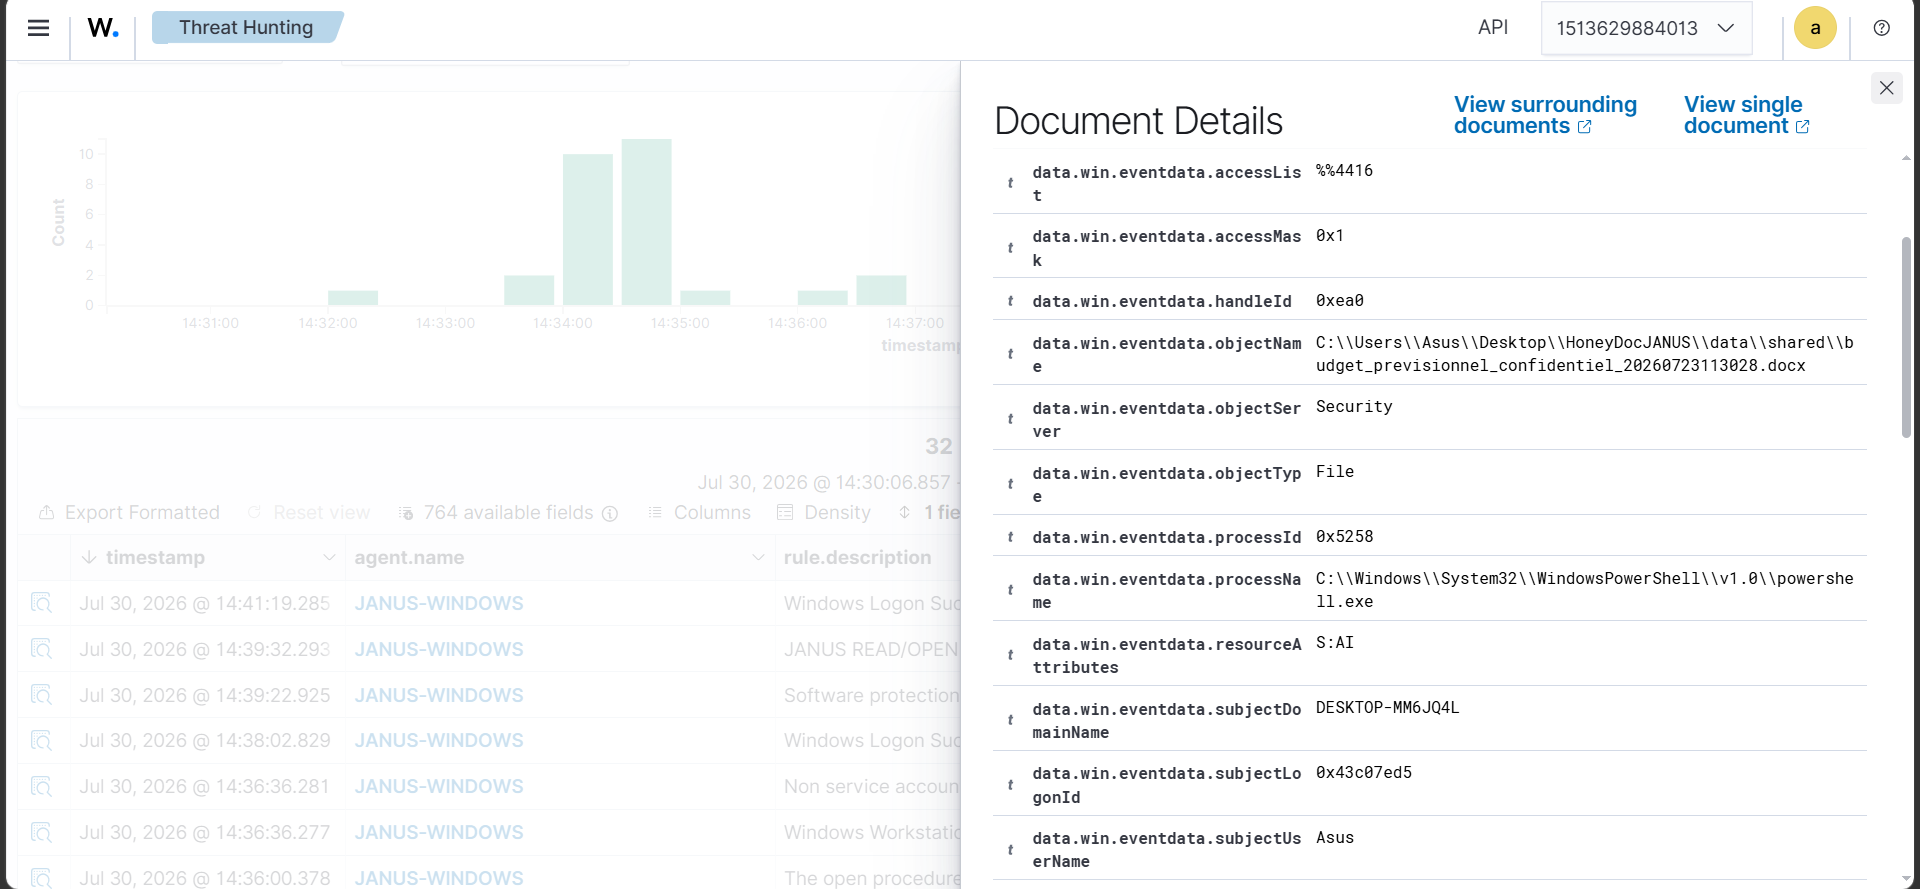
\includegraphics[width=0.95\linewidth]{wazuh-4663-fields.png}
\caption{Event 4663 fields: object, process, access mask, and account}
\label{fig:wazuh-fields}
\end{figure}

\begin{figure}[H]
\centering
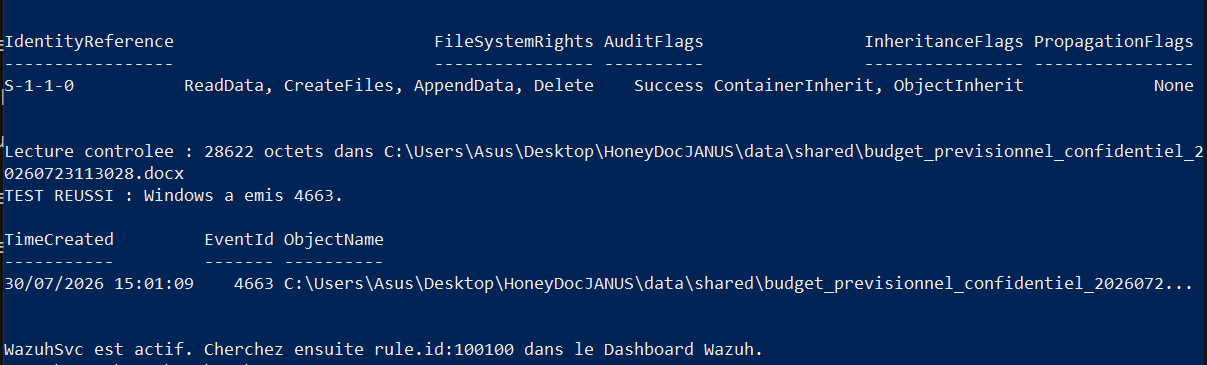
\includegraphics[width=0.95\linewidth]{windows-sacl-4663-test.png}
\caption{Inherited SACL and controlled Windows 4663 test}
\label{fig:sacl-test}
\end{figure}

\begin{figure}[H]
\centering
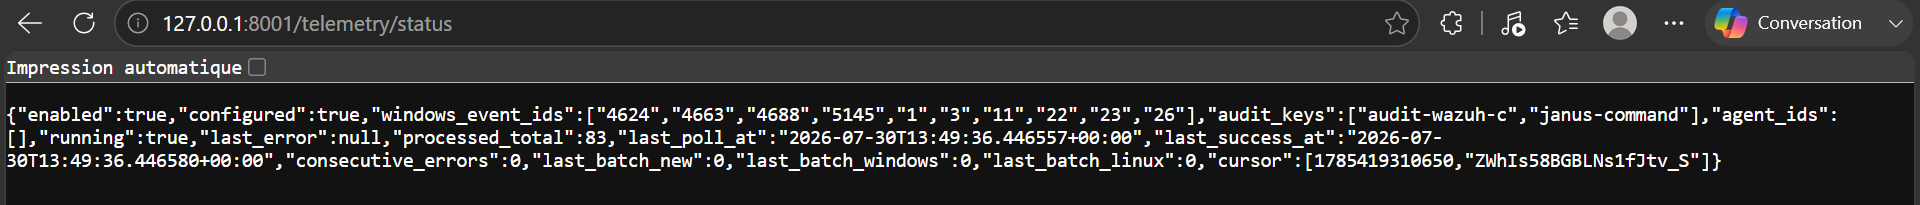
\includegraphics[width=0.95\linewidth]{janus-telemetry-status.png}
\caption{JANUS forensic telemetry status endpoint}
\label{fig:telemetry-status}
\end{figure}

\section{Multi-format and Canarytokens validation}

Manual tests produced valid DOCX, XLSX, JSON, and AWS ENV artifacts. The JSON
selector defect was corrected and verified through the dashboard. An offline
inspection of a newly generated DOCX confirmed one external Office relationship
and no macro. Excel opened the corrected workbook without repair and generated
a Canarytokens email containing a public source IP, provider geolocation, and
the user-agent \texttt{Mozilla/4.0 (compatible; ms-office; MSOffice 16)}. The
exact IP must be redacted in a public report.

The AWS ENV test behaved differently by design. Opening the file produced a
local Wazuh signal but no remote email. The official token is expected to alert
only when the decoy keys are presented to the AWS API.

\begin{table}[H]
\centering
\caption{Observed and expected acceptance results}
\label{tab:acceptance-results}
\small
\begin{tabular}{p{0.22\linewidth}p{0.27\linewidth}p{0.27\linewidth}p{0.16\linewidth}}
\toprule
Scenario & Local Wazuh layer & Remote token layer & Result \\
\midrule
DOCX read & 4663 and read/open rule & Conditional on Word policy & Local validated; remote conditional \\
XLSX opened & File access detected & Office email received & Validated \\
JSON opened & File access detected & No automatic request & Validated behavior \\
AWS ENV opened & File access detected & No activation expected & Validated behavior \\
AWS keys used & Not required on remote host & AWS token email expected, delayed & Manual test to document \\
Modify/delete & Rules 100102/100103 & Not applicable & Supported; repeat for final screenshots \\
\bottomrule
\end{tabular}
\end{table}

\section{Conclusion}

The implementation satisfies the core requirements and demonstrates a complete
local detection path. Remote activation remains format-dependent, which is a
property of the sensors rather than a reason to invent uniform behavior.

\chapter{Evaluation, Limitations, and Evolution}

\section{Introduction}

This chapter evaluates JANUS as a defensive prototype rather than as a
finished commercial product. It separates demonstrated capabilities from
format-dependent behavior and from future work. This distinction is essential
because a deception system loses value when its dashboard reports certainty
that the underlying sensors cannot provide.

\section{Evaluation against the objectives}

\begin{table}[H]
\centering
\caption{Evaluation of the project objectives}
\label{tab:objective-evaluation}
\small
\begin{tabular}{p{0.26\linewidth}p{0.43\linewidth}p{0.21\linewidth}}
\toprule
Objective & Evidence & Status \\
\midrule
Generate varied business decoys & DOCX, XLSX, CSV, JSON, YAML, ENV, and ZIP
artifacts; remote LLM or local fallback & Achieved \\
Prevent unsafe deployment & forbidden-pattern scan, coherence gate,
format inspection, and project-root path policy & Achieved \\
Detect local interaction & inherited SACL, event 4663, Wazuh rules, and
registry correlation & Achieved on Windows \\
Add off-host detection & official Office and AWS token policies with explicit
activation conditions & Partially achieved \\
Preserve evidence & raw alert JSON, Wazuh identifiers, canonical SHA-256, and
normalized signal & Achieved \\
Present honest results & separate local/remote views and explicit confidence
and suppression fields & Achieved \\
Operate as a production SOC platform & high availability, immutable storage,
distributed agents, and production TLS & Out of scope \\
\bottomrule
\end{tabular}
\end{table}

\section{What can be learned about an actor}

The two principal sensors observe different boundaries. Wazuh provides strong
host-side evidence when the file is touched on an enrolled and correctly
audited endpoint. Canarytokens provides a network-side signal after a
format-specific external action. Neither sensor alone identifies a physical
person.

\begin{table}[H]
\centering
\caption{Actor-related information and evidential quality}
\label{tab:actor-evidence}
\small
\begin{tabular}{p{0.24\linewidth}p{0.25\linewidth}p{0.41\linewidth}}
\toprule
Information & Source & Correct interpretation \\
\midrule
Local account and logon identifier & Windows/Wazuh & Direct evidence for the
audited host event; an account may be compromised. \\
Process name and identifier & Windows/Wazuh & Direct evidence for the process
that exercised the audited access right. \\
Object path, access mask, and time & Windows/Wazuh & Direct evidence for the
object and right used at that time. \\
Remote session address or share & 4624/5145 context & Available only when a
compatible session event exists and correlation is justified. \\
Public source IP and time & Canarytokens & Network egress observed by the
provider; a NAT, proxy, or VPN may hide the device. \\
User-Agent and token channel & Canarytokens & Client-claimed protocol metadata;
useful but spoofable. \\
Approximate location and ASN & Provider IP enrichment & Derived from IP
databases, not GPS and not proof of a person's location. \\
MAC address across the Internet & Neither & Unavailable across routed networks
and therefore never generated by JANUS. \\
Remote download from one 4663 event & Neither alone & A read is observed; a
download requires additional SMB, process, or network evidence. \\
Operating system of an unmanaged actor & Neither reliably & A User-Agent may
suggest a client family, but JANUS must label this as an inference. \\
\bottomrule
\end{tabular}
\end{table}

\section{Security and privacy analysis}

JANUS reduces risk through four design choices. First, it never asks the LLM to
generate a real credential and keeps local paths and token secrets out of the
prompt. Second, administrative endpoints require an API key and sensitive
configuration remains outside version control. Third, the generation pipeline
rejects unsafe paths and malformed artifacts before deployment. Fourth, the
evidence layer preserves the provider payload instead of replacing it with an
unverifiable summary.

The same telemetry can contain personal or operational data, including account
names, paths, public IP addresses, and process details. A real deployment must
therefore define access control, retention, lawful purpose, redaction, and
incident-handling rules. Public screenshots must obscure API keys, AWS token
material, email addresses, public IP addresses when unnecessary, and personal
directory names.

\section{Technical limitations}

\subsection{Endpoint visibility}

Wazuh observes only hosts that forward the relevant events. If a HoneyDoc is
copied to a completely unmanaged computer, the original endpoint can show the
access or copy-related context available before departure, but it cannot report
later local activity on the external computer.

\subsection{Office behavior}

Office token activation depends on external-content policy, application
version, Protected View, network controls, and user choices. DOCX opening can
therefore create a reliable local Wazuh event without producing a remote
callback. JANUS does not use macros to bypass this policy.

\subsection{Structured documents}

A JSON, YAML, CSV, or ENV file cannot autonomously make a network request while
remaining passive data. Such a file can still be a useful local decoy. A web
breadcrumb activates only if an actor follows or uses it. AWS credentials
activate only when presented to an AWS API, and the provider may report the
event after a delay \cite{canaryAws}.

\subsection{Laboratory infrastructure}

The validated deployment uses one Windows workstation, a local SQLite database,
and a Docker single-node Wazuh stack. Indexer TLS verification is relaxed for a
local self-signed laboratory certificate. This setting, local process launching,
and SQLite storage must be redesigned before production use.

\section{Threats to validity}

The current experiment demonstrates functional correctness but does not measure
detection probability over a representative attacker population. The observed
Canarytokens IP originated from a controlled test, not from an adversary. File
access performed by PowerShell proves the sensor path, not the behavior of every
Office version. Furthermore, geolocation and User-Agent fields are provider
enrichments whose accuracy is outside JANUS control. Repeated experiments on
separate endpoints and networks are needed before drawing statistical
conclusions.

\section{Proposed evolution}

The next release should preserve the simple, explainable core while improving
deployment quality:

\begin{enumerate}[label=\arabic*.]
  \item expose a public HTTPS callback endpoint with authentication and replay
  protection so remote token events enter the same evidence registry;
  \item enrol a separate Windows victim virtual machine and a Linux endpoint to
  test the trust boundary rather than using only the development host;
  \item enable production certificate verification and secret management;
  \item export JSON/CSV evidence bundles and add role-based dashboard access;
  \item define retention and redaction policies and move evidence to an
  append-only or externally protected store;
  \item measure time-to-detect, false-positive rate, callback rate by format,
  and correlation coverage across repeated scenarios;
  \item add signed deployment manifests and reproducible release packaging.
\end{enumerate}

Experimental fake SSH/HTTP services and prompt-injection or credential-trap
layers should remain outside the core evaluation unless a future research
question explicitly needs them. They are not required for the HoneyDoc plus
Wazuh plus Canarytokens contribution.

\section{Conclusion}

JANUS achieves its academic MVP objective: it creates controlled decoys,
observes a real Windows interaction through Wazuh, supports official remote
token mechanisms, and preserves evidence without inventing attacker
attributes. Its most important future work is not to add more speculative
fields, but to validate the same evidence model on isolated endpoints and to
integrate authenticated remote callbacks.


\chapter*{General Conclusion}
\addcontentsline{toc}{chapter}{General Conclusion}
JANUS demonstrates that AI-generated honey documents can be combined with
endpoint and remote deception sensors in a coherent and testable pipeline. The
generation subsystem creates several document families, selects an official
token type appropriate to the requested format, validates the artifact before
deployment, and records its identity and hash. The detection subsystem
correlates Windows 4663 events with the active decoy registry and preserves raw
evidence. The dashboard then separates local Wazuh detections from remote
Canarytokens callbacks instead of merging unlike signals.

The project also establishes clear limits. Wazuh observes the endpoint on
which its agent and audit policy are active; it cannot follow a copied file on
an unmanaged host. A public Canarytokens notification normally identifies a
requesting network path, not a physical person or device. Office callbacks can
be blocked, and AWS key alerts require actual API use. Within those limits, the
validated prototype provides a sound basis for an academic demonstration and
for future work on public webhook ingestion, distributed deployments, and
measured deception effectiveness.

\bibliographystyle{plain}
\bibliography{refs}

\appendix
\chapter{Acceptance Test Summary}
The complete operational procedure is maintained in
\texttt{docs/MANUAL\_TEST\_GUIDE.md}. The minimum acceptance criteria are:
\begin{enumerate}[label=\arabic*.]
  \item the automated suite passes (98 tests and 7 subtests in the validated build);
  \item Wazuh and forensic collectors report \texttt{running=true} without errors;
  \item a DOCX read produces a correlated 4663 event and rule 100101/100104;
  \item XLSX can produce both a local Wazuh signal and a remote Office token alert;
  \item JSON produces the requested suffix and no false automatic-callback claim;
  \item AWS decoy credentials alert only when presented to the AWS API;
  \item secrets and live token material are absent from screenshots and Git.
\end{enumerate}

\end{document}
